\section{Backgrounding}


\subsection{Common Deep Network BackBone}
Deep convolutional neural networks (CNNs) \cite{Lecun2014Backpropagation} have been widely used in light of their successes in many computer vision tasks, such as, face recognition\cite{Schroff2015FaceNet},  object detection\cite{Ren2015Faster}, and image classification\cite{Krizhevsky2012ImageNet}. CNNs use the multi-layer nonlinear function to approximate the mapping function from input to output.

The famous LeNet contains 5 layers. Later as the enhancement in the computing capability of GPUs, deeper CNNs with more convolutional layers, including AlexNet (8 layers) \cite{Krizhevsky2012ImageNet} and VGGNet (16 layers) (16 layers)\cite{Simonyan-VGG} are proposed. Experimental results show that the increase in depth improves the capability of CNNs for image classification. Fig.\ref{VGG} shows the architecture of VGG.

\begin{figure}[ht]
    \centering
    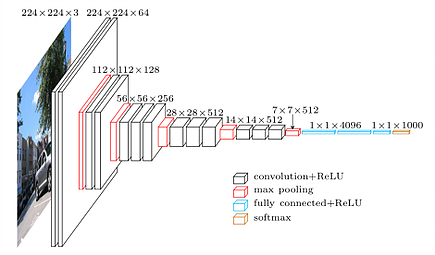
\includegraphics[width=0.5\textwidth]{./figure/VGG.png}
    \caption{VGG Network}
    \label{VGG}
\end{figure}

In GoogLeNet\cite{Szegedy-GoogLeNet}, Szegedy \etal propose the `\emph{Inception module}', which is aimed to find out an optimal local sparse structure in a convolutional network. The Inception architecture vision contains three paths with filters sizes $1 \times 1$, $3 \times 3$ and $5\times 5$, an alternative parallel pooling path, and a combination of all those layers with their output filter banks concatenated into a single output vector forming the input of the next stage.
Such an Inception network is a network consisting of modules of such type stacked upon each other, with occasional max-pooling layers with stride 2 to decrease the resolution of the grid.
Compared with AlexNet \cite{Krizhevsky2012ImageNet}, VGGNet\cite{Simonyan-VGG}, GoogLeNet\cite{Szegedy-GoogLeNet}, ResNet is a more deeper framework with residual learning strategy designed by He \etal in \cite{He-Resnet}. ResNet is neural networks in which each layer consists of a residual module $f_i$ and a skip connection bypassing $f_i$.
In \cite{veit2016residual}, Veit \etal propose a new interpretation of residual networks, which shows residual networks can be seen as a collection of many paths of differing length.
In \cite{xie2017aggregated}, Xie \etal propose a highly modularized network architecture named `\emph{ResNeXt}' and introduces a dimension `\emph{cardinality}' as a factor to the dimensions of depth and width. A module in ResNeXt performs a set of transformations each on a low-dimensional embedding, whose outputs are aggregated by summation and the transformations to be aggregated are all of the same topology.
In \cite{huang2016densely}, Huang \etal design the Dense Convolutional Network (DenseNet), which connects each layer
to every other layer in a feed-forward way. For each layer, the feature-maps of all preceding layers are used as inputs, and its own feature-maps are used as inputs into all subsequent layers.

\begin{figure}[ht]
    \centering
    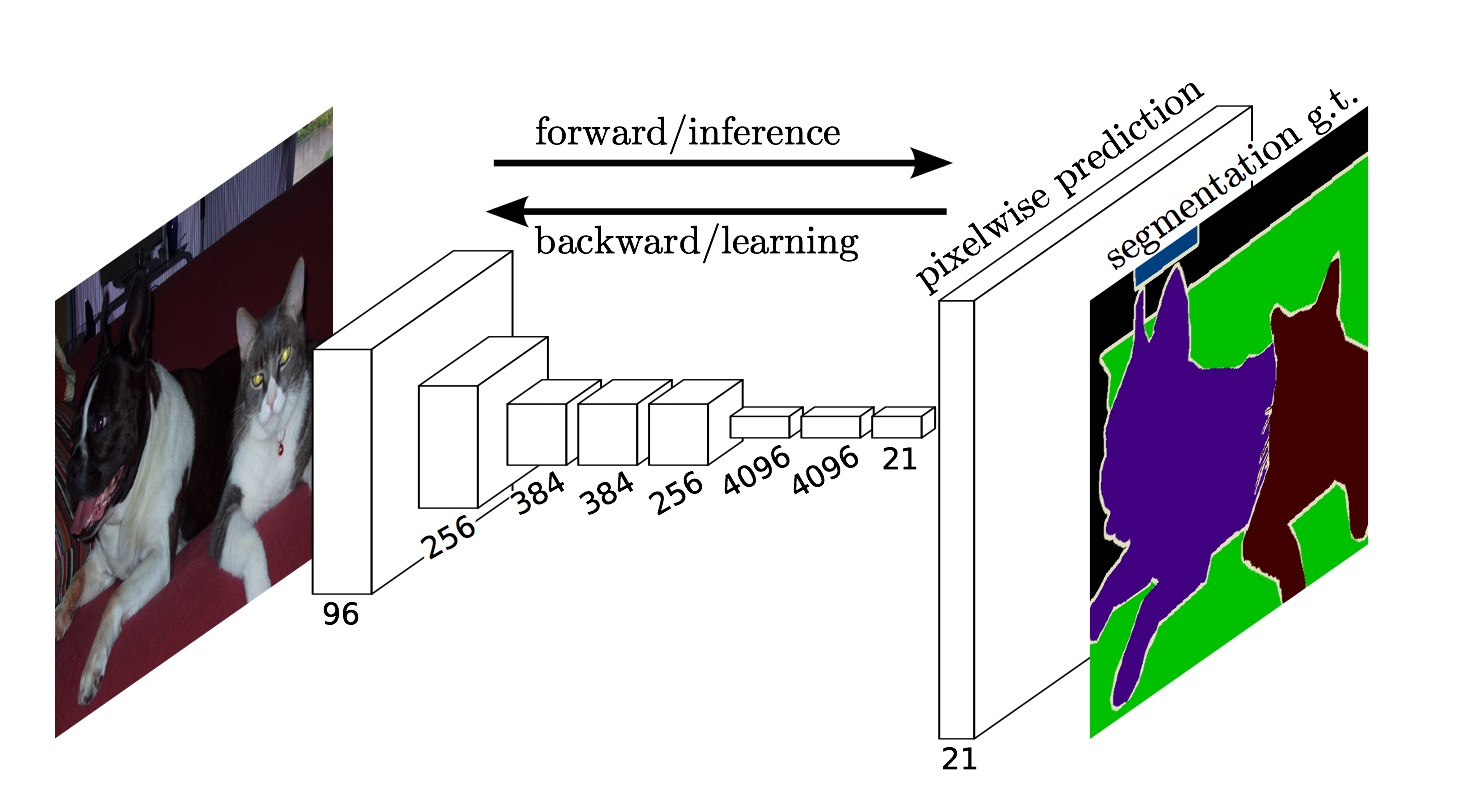
\includegraphics[width=0.5\textwidth]{./figure/FCN.png}
    \caption{FCN framework}
    \label{FCN}
\end{figure}

\subsection{Common Deep Network Architecture}
\subsubsection{FCN}
Semantic pixel-wise segmentation is an active topic of research. Recently, CNNs also have been introduced to solve segmentation problem. 

In \cite{Long2015Fully}, Long \etal define and detail the space of fully convolutional networks, which take input of arbitrary size and produce correspondingly-sized output with efficient inference and learning. A skip architecture is also designed that combines semantic information from a deep, coarse layer with appearance information from a shallow, fine layer to produce accurate and detailed segmentations. 


\subsubsection{SegNet}
In \cite{SegNet}, Badrinarayanan \etal present a deep fully convolutional neural network architecture for semantic pixel-wise segmentation termed SegNet, which consists of an encoder network, a corresponding decoder network followed by a pixel-wise classification layer. The role of the decoder network is to map the low resolution encoder feature maps to full input resolution feature maps for pixel-wise classification. Specifically, the decoder uses pooling indices computed in the max-pooling step of the corresponding encoder to perform non-linear upsampling.

\begin{figure}[ht]
    \centering
    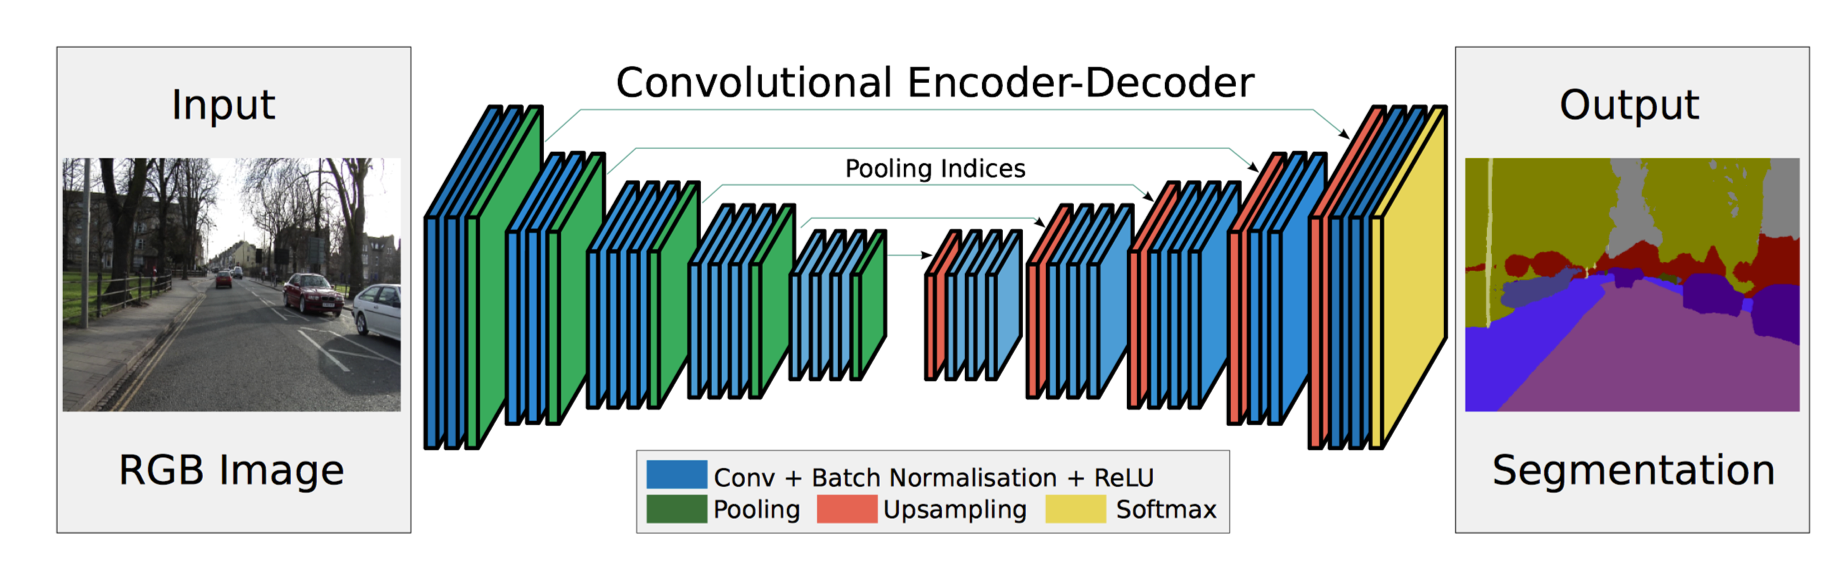
\includegraphics[width=0.5\textwidth]{./figure/SegNet.png}
    \caption{SegNet framework}
    \label{SegNet}
\end{figure}

\subsubsection{U-Net}
Ronneberger \etal propose U-Net for biomedical image segmentation in \cite{Ronneberger2015U}. The architecture of U-Net consists of a contracting path to capture context and a symmetric expanding path that enables precise localization. 
In the upsampling part, U-Net has also a large number of feature channels, which allow the network to propagate context information to higher resolution layers. As a consequence, the expansive path is more or less symmetric to the contracting path, and yields a u-shaped architecture.

\begin{figure}[ht]
    \centering
    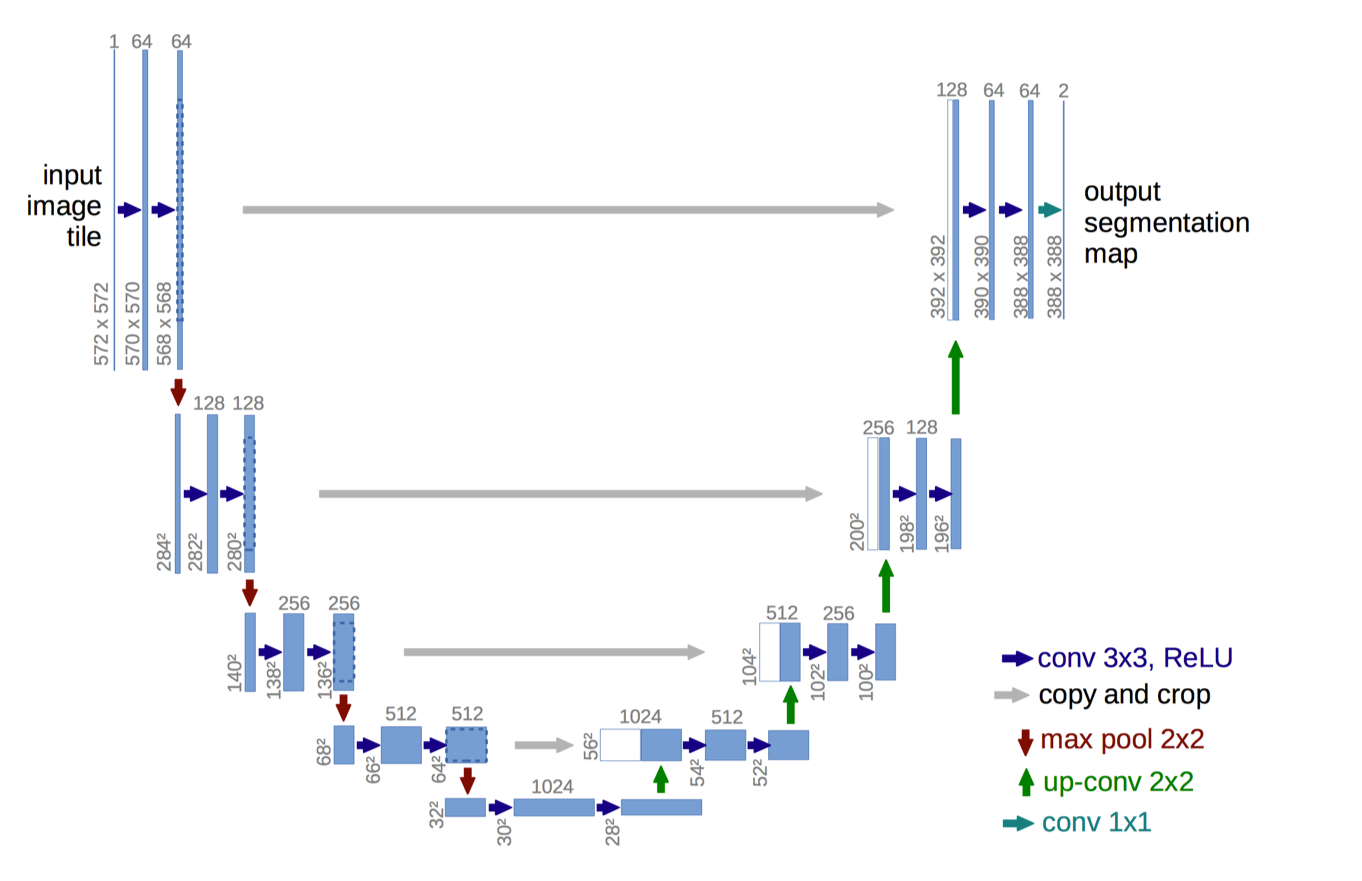
\includegraphics[width=0.5\textwidth]{./figure/unet.png}
    \caption{U-Net framework}
    \label{unet}
\end{figure}

\subsection{Common Method for Video}

\subsubsection{Optical Flow}
Optical flow or optic flow is the pattern of apparent motion of objects, surfaces, and edges in a visual scene caused by the relative motion between an observer and a scene.The concept of optical flow was introduced by the American psychologist James J. Gibson in the 1940s to describe the visual stimulus provided to animals moving through the world.\cite{OpticalFlow} Gibson stressed the importance of optic flow for affordance perception, the ability to discern possibilities for action within the environment. Followers of Gibson and his ecological approach to psychology have further demonstrated the role of the optical flow stimulus for the perception of movement by the observer in the world; perception of the shape, distance and movement of objects in the world; and the control of locomotion. Fig. \ref{optical flow} shows that an example of optical flow with L2-norm for motion estimation. 

\begin{figure}[ht]
    \centering
    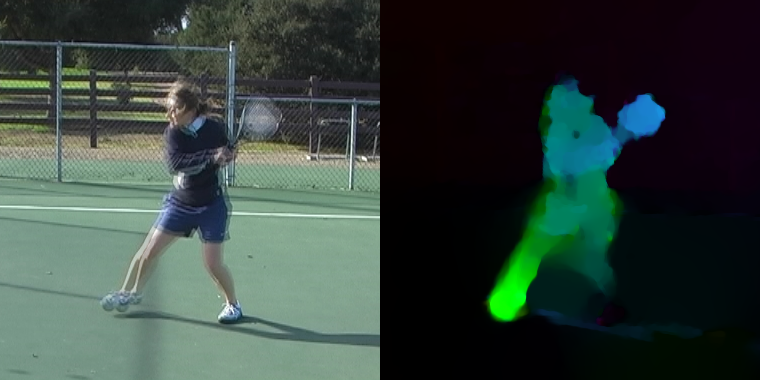
\includegraphics[width=0.5\textwidth]{./figure/opticalflow.png}
    \caption{Optical flow with L2-norm}
    \label{optical flow}
\end{figure}

Video object segmentation is challenging due to fast moving objects, deforming shapes, and cluttered backgrounds. optical flow can be used to propagate an object segmentation over time but, unfortunately, flow is often inaccurate, particularly around object boundaries. Such boundaries are precisely where we want our segmentation to be accurate. To obtain accurate segmentation across time.  Tsai \etal propose an efficient algorithm\cite{OFL}  that considers video segmentation and optical flow estimation simultaneously, formulate a principled, multiscale, spatio-temporal objective function that uses optical flow to propagate information between frames. For optical flow estimation, particularly at object boundaries.they show that segmentation results can be used to refine the optical flow, and vice versa, in the proposed object flow algorithm, and can be efficiently computed by iterative optimization.


\begin{figure*}
    \begin{center}
        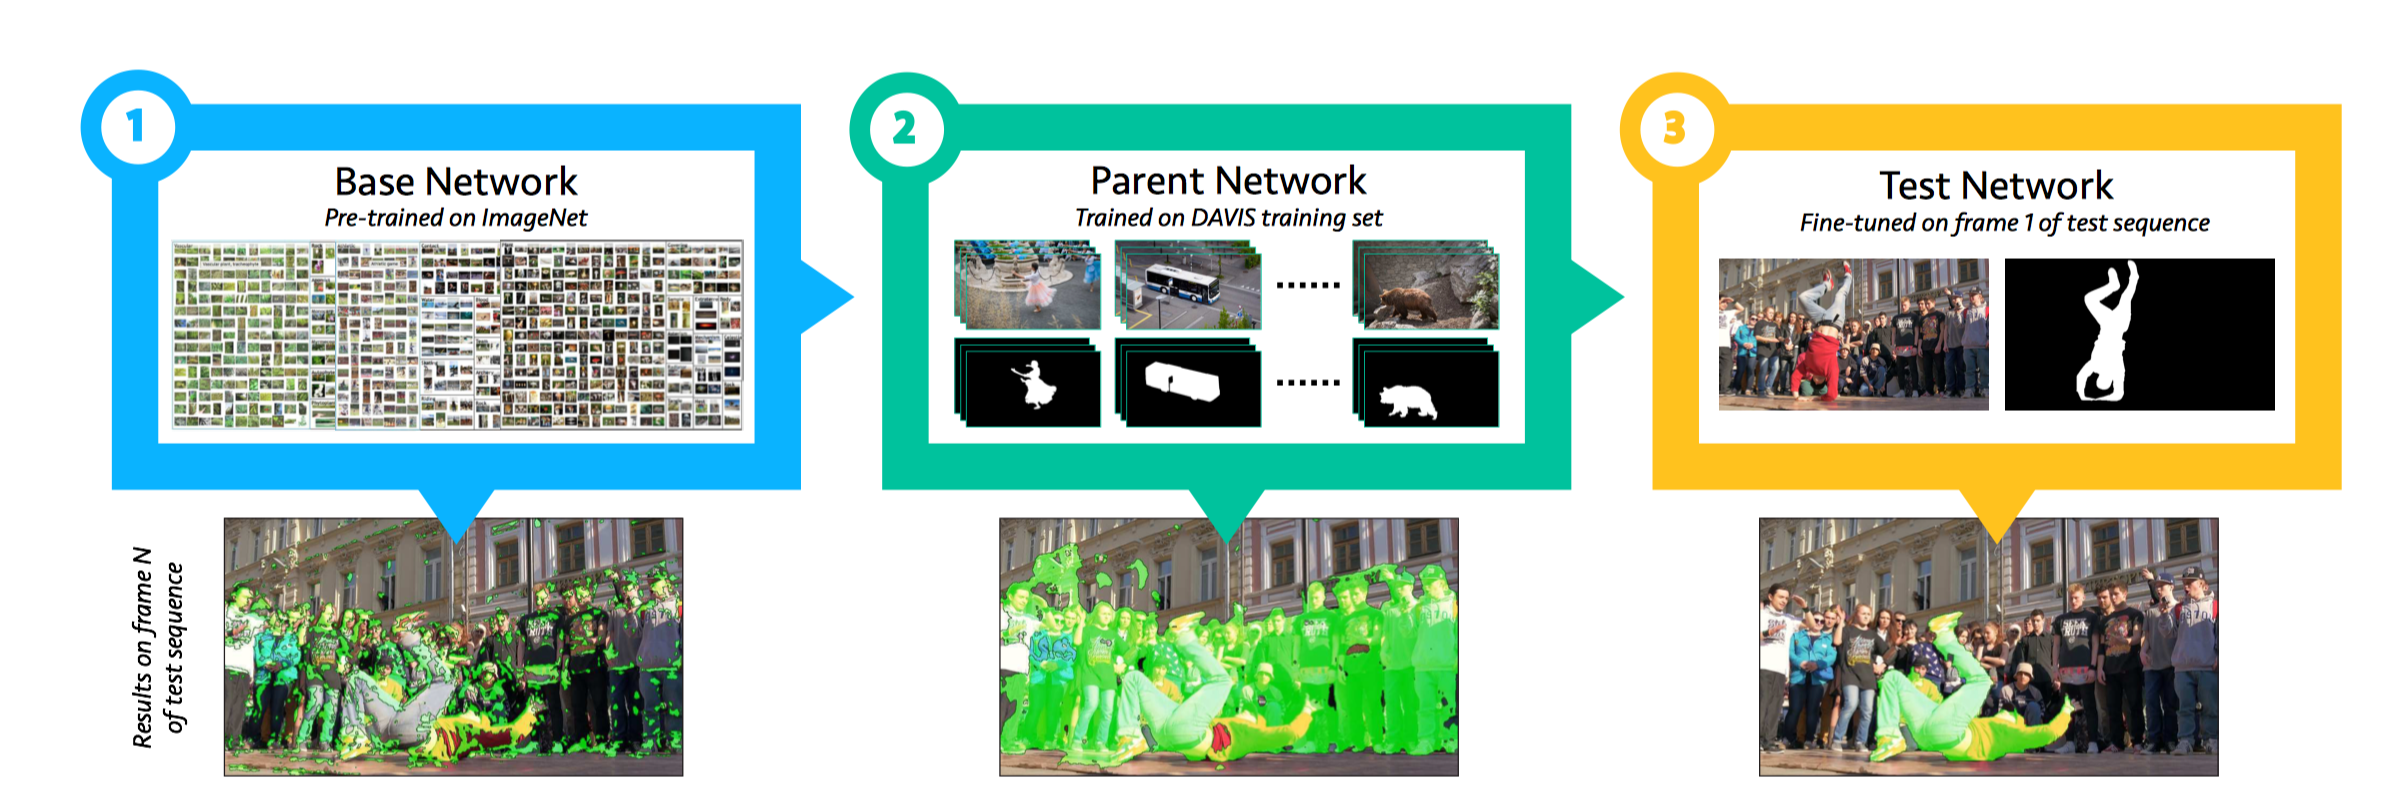
\includegraphics[width=\textwidth]{figure/fine_tune.png}
    \end{center}
    \caption{Fine Tune Method Pipline}
    \label{fine_tune}
\end{figure*}


\subsubsection{Mask Warp}
Mask Warp\cite{LucidTracker} use flow in two complementary ways. First, to obtain a better initial estimate of $M_t$ it warp $M_{t−1}$ using the flow $\mathcal{F}_t : M_t = f_I (\mathcal{I}_t , w(M_{t-1} , F_{t}))$, then use flow as a direct source of information about the mask $M_t$.When the object is moving relative to background, the flow magnitude $||\mathcal{F}_t||$ provides a very reasonable estimate of the mask $M_t$.Consider using a convnet specifically for mask estimation from flow:$M_t = f_{\mathcal{F}} (\mathcal{F}_t , w(M_{t-1} , \mathcal{F}_t))$, and merge it with the image-only version by naive averaging:
\begin{align*}
    M_t = 0.5 * f_I(I_t, ...) + 0.5 * f_\mathcal{F}(\mathcal{F}_t, ...)
\end{align*}

\subsection{Common Method for One-Shot}

\subsubsection{Fine-Tune}
Let us assume that one would like to segment an object in a video, for which the only available piece of information is its foreground/background segmentation in one frame. Intuitively, one could analyze the entity, create a model, and search for it in the rest of the frames. For humans, this very limited amount of information is more than enough, and changes in appearance, shape, occlusions, etc. do not pose a significant challenge, because we leverage strong priors: first “It is an object,” and then “It is this particular object.” Our method is inspired by this gradual refinement.

Fine-Tune method \cite{OSVOS} \cite{OSVOS-S} \cite{OnAVOS} train a BackBone Fully Convolutional Neural Network (BFCN) for the binary classification task of separating the foreground object from the background, Then use two successive training steps: First train on a large variety of objects offline, to construct a model that is able to discriminate the general notion of a foreground object, i.e., “It is an object.” Then, at test time, fine-tune the network for a small number of iterations on the particular instance that we aim to segment, i.e., “It is this particular object.” The overview of our method is illustrated in Fig.\ref{fine_tune}.

\subsubsection{Data Dreaming}
To train the video segmentation network one would think of using ground truth data for $M_{t−1}$ and $M_t$ (like \cite{OSVOS}, \cite{bertinetto2016fully}, \cite{held2016learning}), however such data is expensive to annotate and rare. \cite{OSVOS} thus trains on a set of 30 videos (∼ 2k frames) and requires the model to transfer across multiple tests sets. \cite{Perazzi2017Learning} side-steps the need for consecutive frames by generating synthetic masks $M_{t-1}$ from a saliency dataset of ∼ 10k images with their corresponding mask $M_t$ . Data Dreaming Method\cite{LucidTracker} propose a new data generation strategy to reach better results using only ∼100 individual training frames.

\begin{figure}[ht]
    \centering
    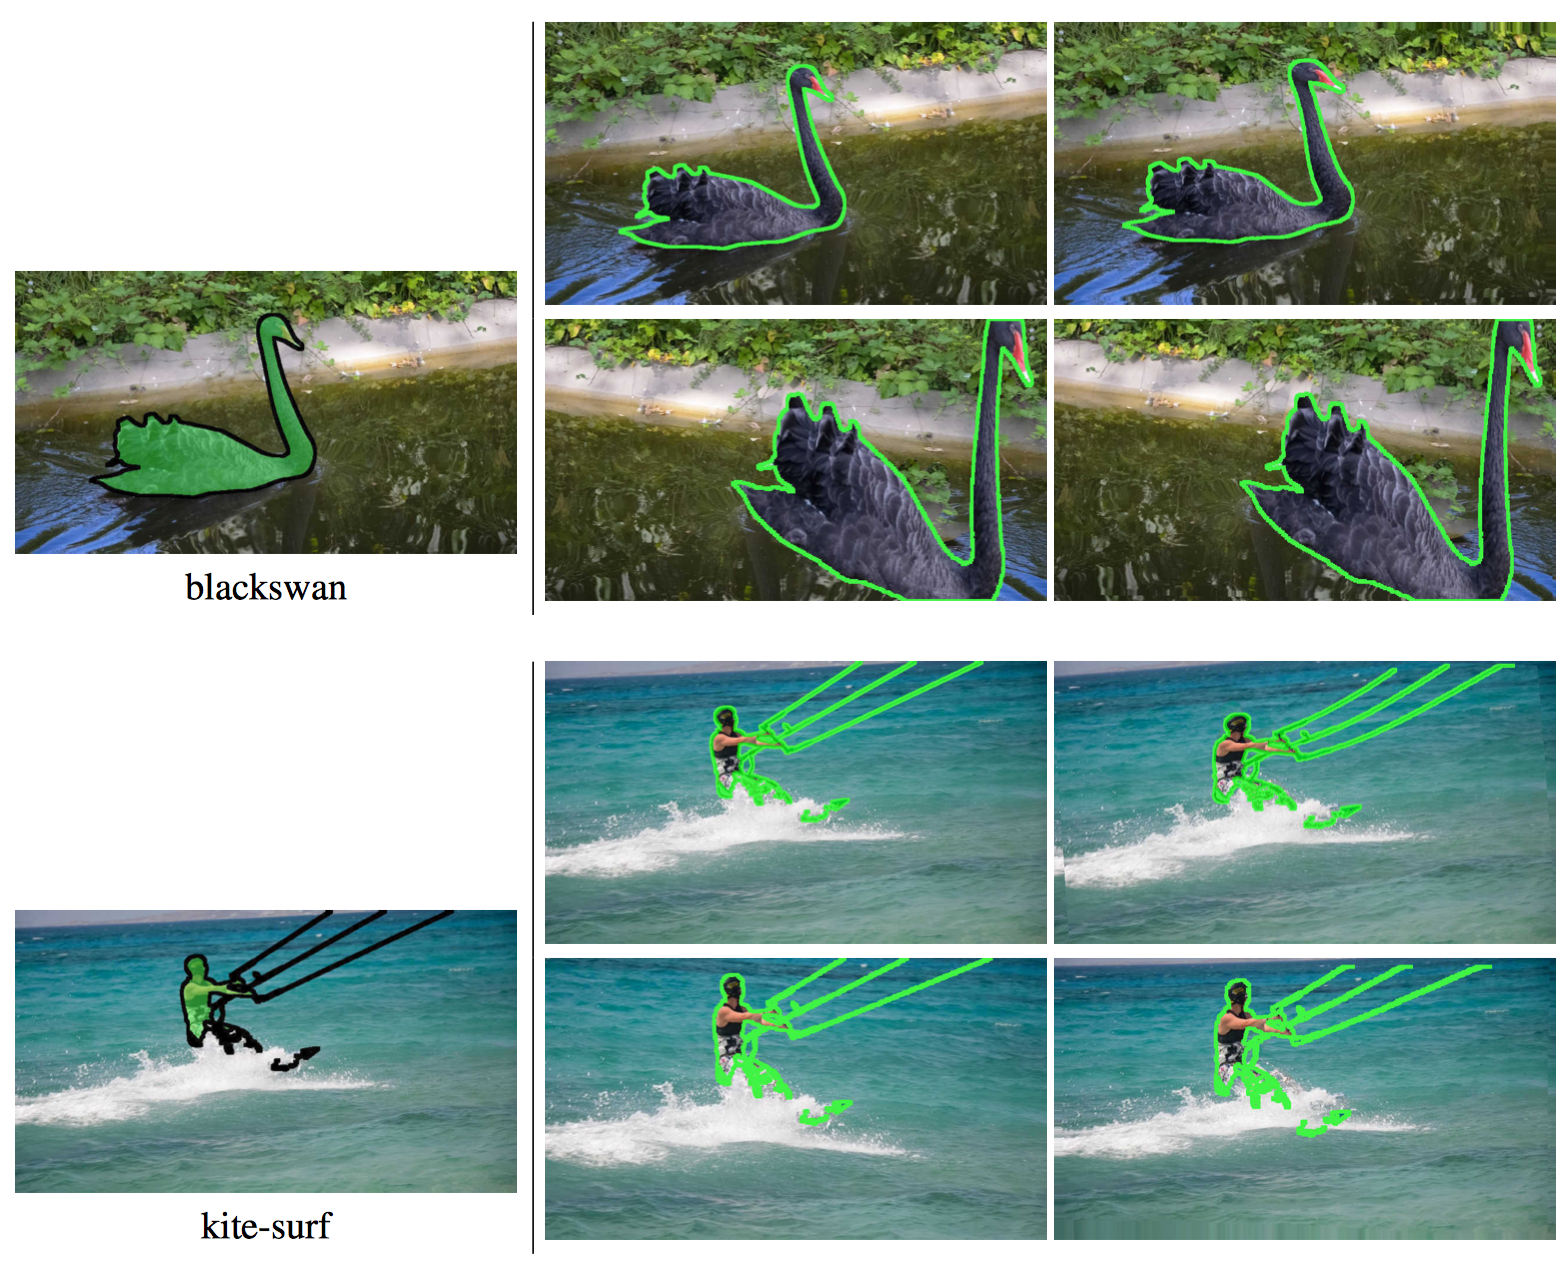
\includegraphics[width=0.5\textwidth]{./figure/data_dream.png}
    \caption{Data Dream on DAVIS-2016 Sequence}
    \label{data dream}
\end{figure}


Ideally training data should be as similar as possible to the test data, even subtle differences may affect quality (e.g. training on static images for testing on videos under-performs \cite{tang2012shifting}). To ensure our training data is in-domain, \cite{LucidTracker} propose to generate it by synthesizing samples from the provided annotated frame (first frame) in each target video. This is akin to “lucid dreaming” as we intentionally “dream” the desired data by creating sample images that are plausible hypothetical future frames of the video. The outcome of this process is a large set of frame pairs in the target domain (2.5k pairs per annotation) with known optical flow and mask annotations, see Fig.\ref{data dream}.

